\section{Evaluation}
\label{sec:eval}
We evaluated both GEHL and O-GEHL in a variety of ways across all of the traces provided by the course staff.  For GEHL we examined how the history length (as determined by $\alpha$ and $L1$), the value of $\theta$, the number of bits used for the saturating counters and the number of tables affect the prediction accuracy.  For O-GEHL, we examined the impact of dynamically adjusting the history length as well as dynamically adjusting the value of $\theta$.  In addition to predictor accuracy, we also see how various predictors affect the IPC using a simulation of a super-scalar out of order processor.  When appropriate, we compared GEHL and O-GEHL against a variety of baseline predictors.

Due to time constraints, we did not run our simulations on all of the microops in all of our benchmarks.  Instead, we created a short and long version for each trace and for each experiment, chose one or the other.  Details about the traces we used, as well as their lengths, are in Table\ref{table:traces}.  In each of our figures, average accuracies are reported as the unweighted mean across all traces that were used.
\begin{table}
  \centering
  \begin{tabular}{l|r|r|r}
    Trace Name & Total Operations & Long Version & Short Version \\ \hline
    gcc & 50M & 50M & 10M \\
    go & 100M & 100M  & 10M \\
    hmmer & 100M & 100M & 10M \\
    libquantum & 100M & 50M & 10M\\
    sjeng & 100M &50M & 10M \\
    sphinx3 &100M & 50M & 10M \\
    art & 100M & 50M & 10M\\
    mcf & 100M & 100M & 10M\\
 \end{tabular}
 \caption{Traces used throughout the experiments.  Depending on the experiment, either a version with a larger number of microops was used or one with a shorter number of operations was used.}
 \label{table:traces}
\end{table}

Overall our results agree with those reported by Seznec.\cite{seznec2005analysis}\cite{ogehl}

\subsection{Prediction accuracy against baseline predictors}
In order to compare the prediction accuracies of various predictors, we ran
each of them across the traces by varying the cache sizes. Long version of
traces are used in this experiments, of which each trace is at the size of 50M
or 100M. For GEHL and O-GEHL, we use the best parameters getting from our
experiments, namely, the number of table used is around 6, the $\alpha$ is set
to 2, and the saturating counter width is set to 4.From the results, we could
infer that as the cache size increases, the GEHLand the O-GEHL predictors
outperform all of the other predictors. For instance, O-GEHL's performance is
the best of all predictors we've compared when the predictor size is bigger
than 4K-bit. Although we did not perform the experiments on very long traces,
we expect the O-GEHL predictor to eventually outperform all predictors since
its begins exploiting very long global histories.  See
Figure~\ref{fig:comparison} for full results.
\begin{figure}[h]

  \subfigure[Branch predictor accuracy (long traces)]
  {\label{subfig:graph1-acc}\scalebox{0.8}{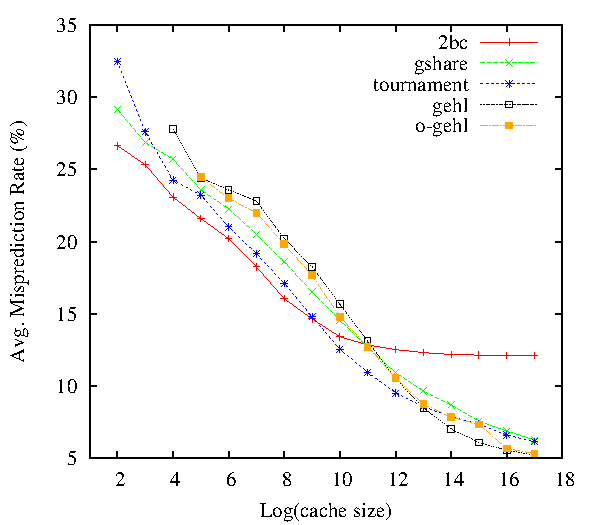
\includegraphics{figs/graph1-acc.pdf}}}
  \subfigure[Standard deviation of predictor accuracy.]
  {\label{subfig:graph1-stddev}\scalebox{0.8}{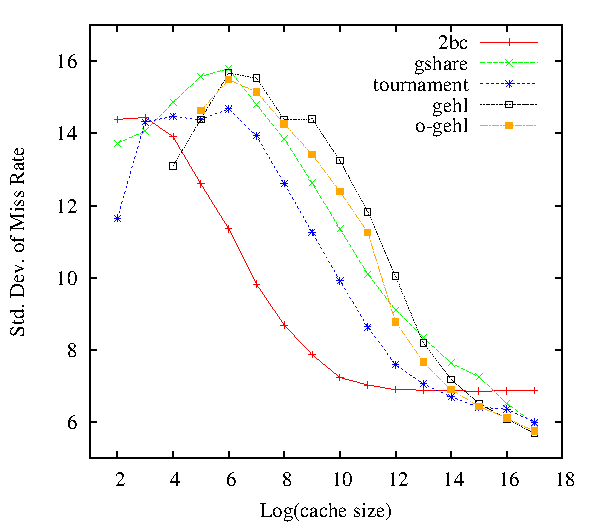
\includegraphics{figs/graph1-stddev.pdf}}}

  \subfigure[Branch predictor accuracy (long traces)  Zoomed in.]
  {\label{subfig:graph1-acc-zoom}\scalebox{0.8}{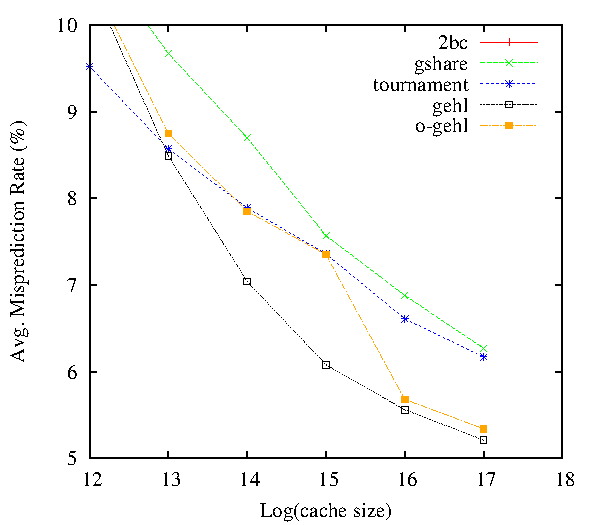
\includegraphics{figs/graph1-acc-zoom.pdf}}}
  \subfigure[Standard deviation of predictor accuracy. Zoomed in.]
  {\label{subfig:graph1-stddev-zoom}\scalebox{0.8}{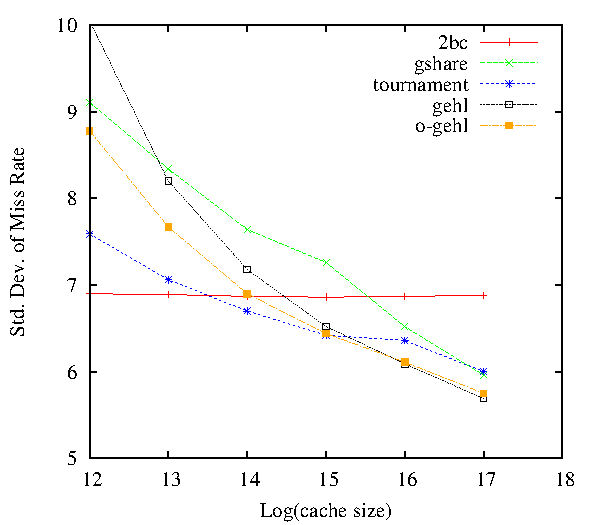
\includegraphics{figs/graph1-stddev-zoom.pdf}}}

  \caption{Branch predictor compassion.  Each data point in \ref{subfig:graph1-stddev} reports the standard deviation of the accuracy of the same predictor in \ref{subfig:graph1-acc}.  \ref{subfig:graph1-acc-zoom} and \ref{subfig:graph1-stddev-zoom} show a closeup of the large predictors' performance.  Overall GEHL outperforms O-GEHL until large predictor sizes are reached, at which point O-GEHL does about as well.  However, they both outperform the other branch predictors.}
  \label{fig:comparison}
\end{figure}

\subsection{Update threshold}
As discussed in Section~\ref{sec:gehl}, GEHL updates when a misprediction occurs or when the magnitude of the sum from all of the tables is below a threshold $\theta$.  Figure~\ref{fig:theta} shows several GEHL predictors across various sizes and with various values of $\theta$.  In the range that we explored, $\theta$ doesn't have a significant impact on the average accuracy.  However, a more detailed analysis of our results show that the best value of $\theta$ varies from trace to trace, just as Seznec indicated. Table 2 shows the best $\theta$ value in our experiments for a 1-Kbit GEHL predictor.
\begin{table}
  \centering
  \begin{tabular}{l|r}
    Trace Name(Short Version) & Best $\theta$ \\ \hline
    gcc & 8 \\
    go &  10 \\
    hmmer &10 \\
    libquantum & 4\\
    sjeng  & 4\\
    sphinx3  &4 \\
    art  &10\\
    mcf  & 10\\
 \end{tabular}
 \caption{$\theta$ with best performance for a 1-Kbit GEHL predictor of each trace.}
 \label{table:bestTheta}
\end{table}
\begin{figure}[h]
  \subfigure[Branch predictor accuracy (short traces)]
  {\scalebox{0.8}{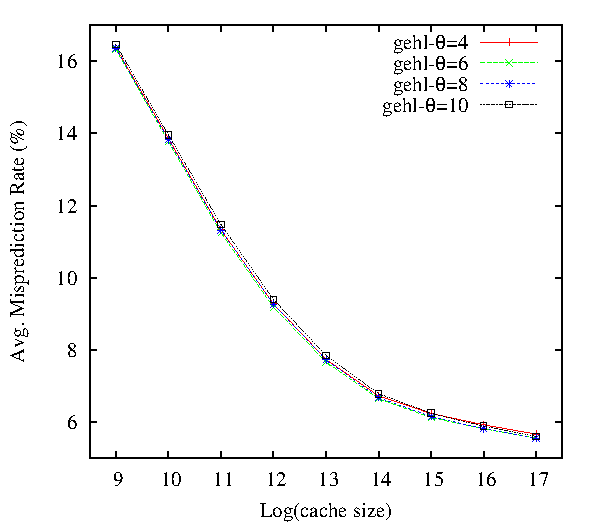
\includegraphics{figs/graph2-acc.pdf}}}
  \subfigure[Standard deviation of branch predictor accuracy]
  {\scalebox{0.8}{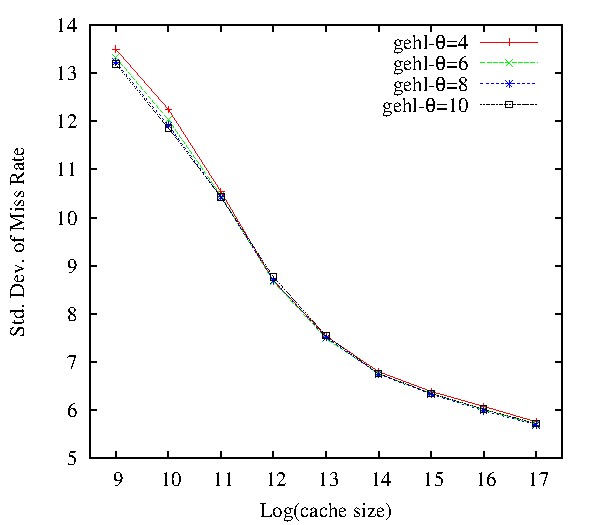
\includegraphics{figs/graph2-stddev.pdf}}}

  \caption{How the value of $\theta$ affects GEHL's prediction accuracy.  Overall, $\theta$ does not have a substantial affect on the accuracy of the branch predictors.}
  \label{fig:theta}
\end{figure}


\subsection{Size of Saturating Counters}
Determining the best size of the saturating counters for a GEHL predictors is a tradeoff between space complexity and performance. Figure~\ref{fig:sb} shows our experimental results for saturating counters with various widths. Performance improves significantly when the the counter increases from from 3-bits to 4-bits.  The standard deviation also drops significantly, indicating that the predictor performs much better across all traces.  However, the performance gain of using 5 bits or more is limited, whereas the added size is substantial as each entry of each table uses a counter.  This data suggests that using 4-bit counters is a good tradeoff.  Seznec reported similar results.

\begin{figure}[h]
  \subfigure[Branch predictor accuracy (short traces)]
  {\scalebox{0.8}{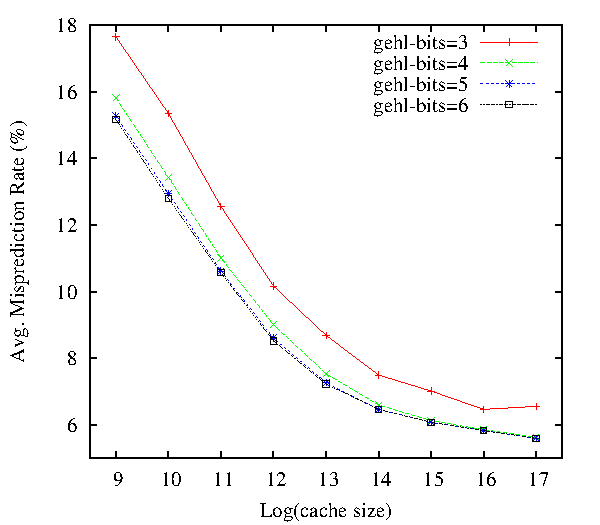
\includegraphics{figs/graph3-acc.pdf}}}
  \subfigure[Standard deviation of branch predictor accuracy]
  {\scalebox{0.8}{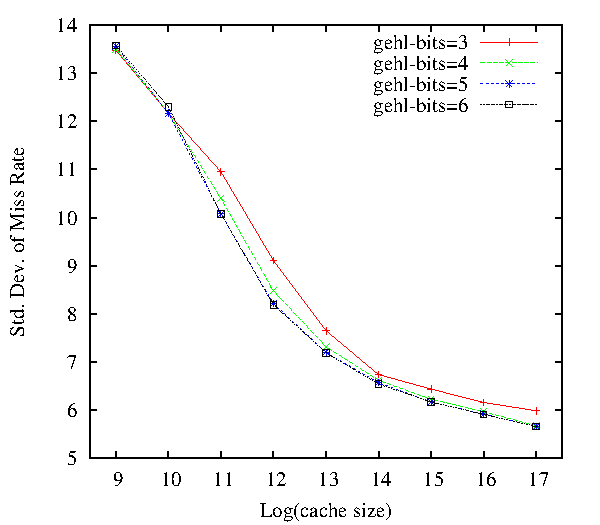
\includegraphics{figs/graph3-stddev.pdf}}}

  \caption{How the size of each table's saturating counters affect GEHL's prediction accuracy.}
  \label{fig:sb}
\end{figure}


\subsection{History length}
The length of each history table used in GEHL is determined by a geometric series based on $\alpha$. From Figure~\ref{fig:alpha}, we see that $\alpha=2.0$ gives the best results for all sizes of the cache.  Smaller values of $\alpha$, such as 1.2 work well when the storage budget is around 1K bits, and large $\alpha$, such as $\alpha$ = 3.0 gives competitive accuracy when the cache size is larger than 16 Kbits. This finding corresponds with Seznec's work as well.  It is worth mentioning that these experiments were done using 6 tables.  If this number had been larger, using a smaller $\alpha$ may have been advantageous because it would capture a finer range of history lengths.
\begin{figure}[h]
\subfigure[Branch predictor accuracy (short traces)] {\scalebox{0.8}{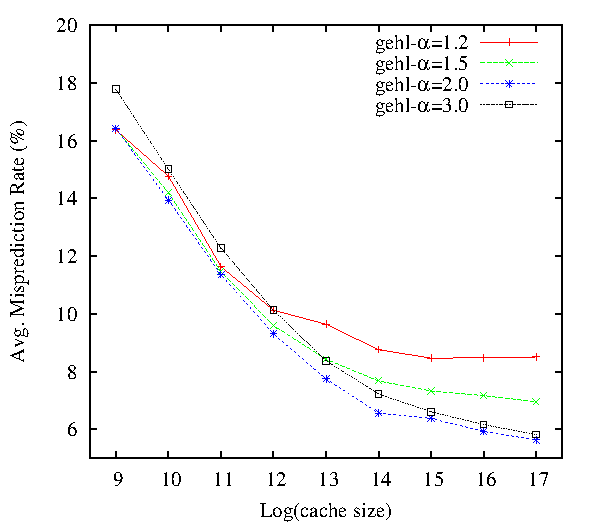
\includegraphics{figs/graph4-acc.pdf}}}
\subfigure[Standard deviation of branch predictor accuracy]
{\scalebox{0.8}{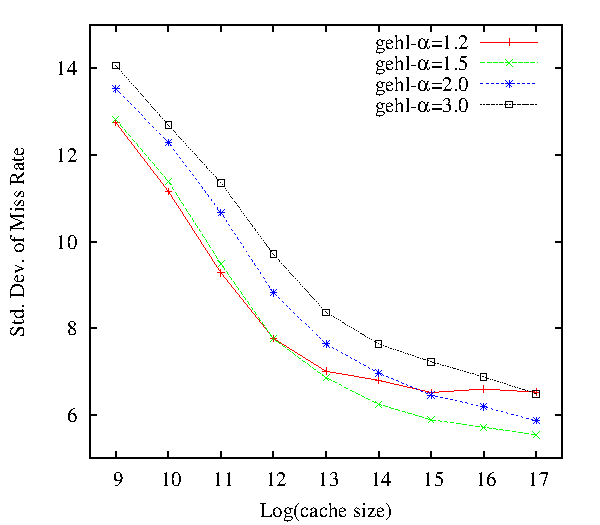
\includegraphics{figs/graph4-stddev.pdf}}}

\caption{How $\alpha$, the growth rate of the history length, affects GEHL's prediction accuracy.}
\label{fig:alpha}
\end{figure}

\subsection{Number of Tables}
The number of tables has the single greatest impact on the performance and space complexity of the predictors.  Figure~\ref{fig:tables} contains data for a wide range of table sizes.  The number of index bits used in the predictor was adjusted to insure relevant comparisons between predictors.  For the set of considered benchmark traces, we found 6 tables to perform the best when the predictor storage budget was small (less than or equal to 96 Kbits).  For such a storage budget, doubling the number of predictor tables, but halving each individual table indexing bits does not improved any performance.  When the storage budget is very small (less than 16Kbits), a 4 table configuration outperforms than 6 table configuration.  Not surprisingly, the general trend is that for large storage budgets, using more tables results in higher accuracy.

\begin{figure}[h]
  \subfigure[Branch predictor accuracy (short traces)]
  {\scalebox{0.8}{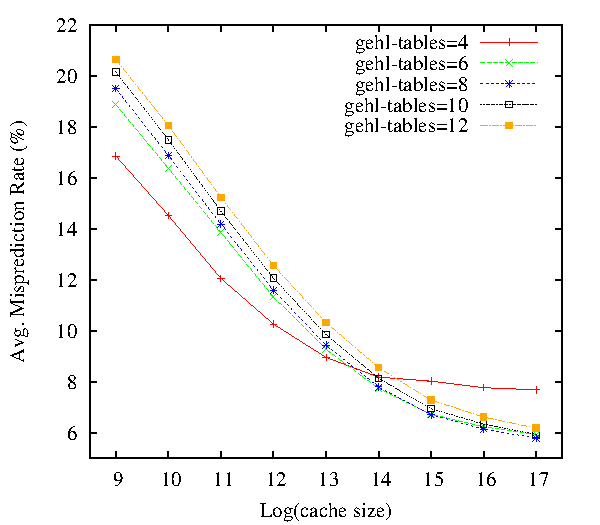
\includegraphics{figs/graph5-acc.pdf}}}
  \subfigure[Standard deviation of branch predictor accuracy]
  {\scalebox{0.8}{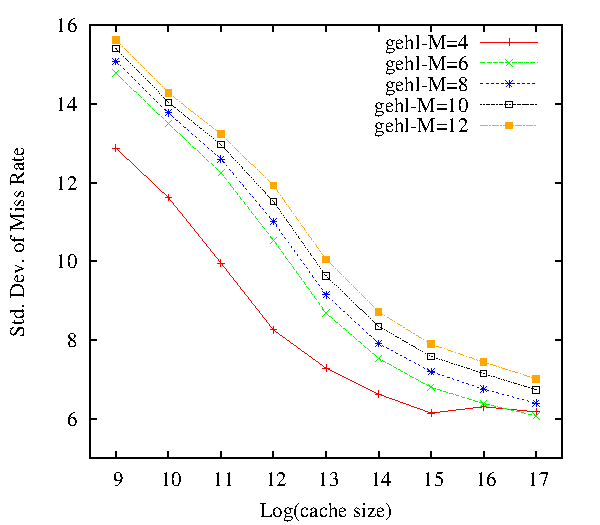
\includegraphics{figs/graph5-stddev.pdf}}}
  \caption{How the number of tables affects GEHL's prediction accuracy.}
  \label{fig:tables}
\end{figure}

\subsection{Adaptive Update Threshold and Adaptive History Length}
Two important changes were introduced in optimizing the original GEHL to O-GEHL.  One is the dynamic threshold fitting policy and the other is adaptive history length.  As we described in Section~\ref{sec:adaptT}, the best value of $\theta$ varies from trace to trace. Figure~\ref{fig:adaptT} shows a comparison between two GEHL predictors with different values of $\theta$ as well as an O-GEHL predictor which dynamically updates the threshold.  In general, O-GEHL performs about as well as the best fixed $\theta$ for each trace. In order to insure that the differences in performance were only due to adjustments of $\theta$, we disabled the dynamic history component of O-GEHL to collect this data.

Figure~\ref{fig:adaptH} shows a comparison between an O-GEHL predictor which adapts its history length as described in Section~\ref{sec:adaptH} and two separate GEHL predictors with vastly different history lengths.  In our experiment, though dynamically fitting history length reduces space complexity, its performance is not better than our best fixed history length growth rate $\alpha=2.0$. This is mainly because history information is lost during our indexing information extraction process, which we discussed in Section~\ref{sec:indexing}.

\begin{figure}[h]
  \centering
  \scalebox{0.8}{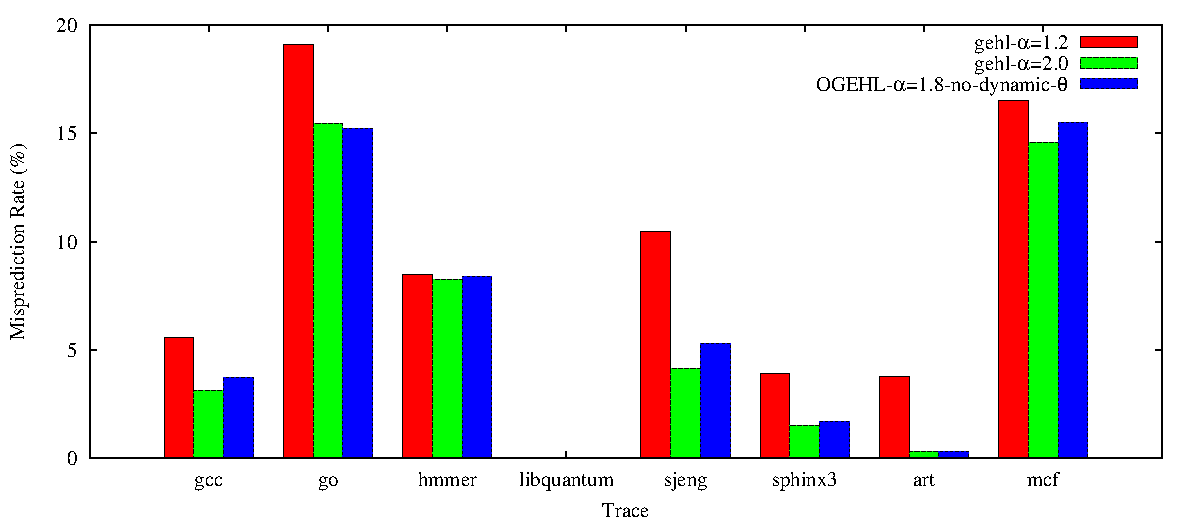
\includegraphics{figs/graph6.pdf}}

  \caption{Performance of O-GEHL with adaptive history length.  Adaptive $\theta$ is not used.  Adaptive history length is not used. All other parameters are the same and each of the predictors is 64Kbits.  This data was collected on the short traces.}
 \label{fig:adaptH}
\end{figure}

\begin{figure}[h]
  \centering
  \scalebox{0.8}{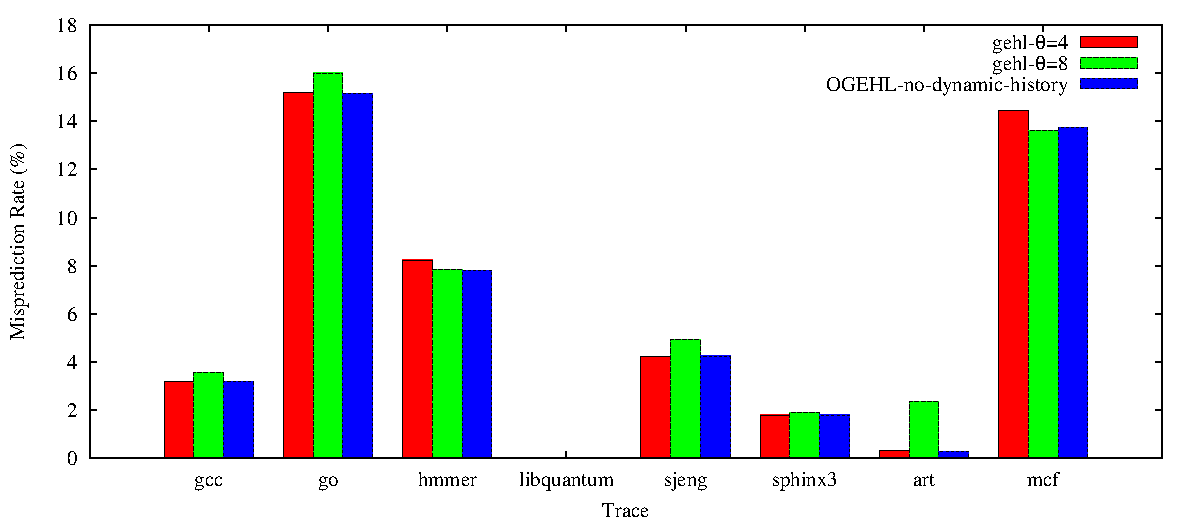
\includegraphics{figs/graph7.pdf}}

  \caption{Performance of OGEHL with adaptive $\theta$.  Adaptive history length is not used. All other parameters are the same and each of the predictors is 64Kbits.  This data was collected on the short traces.}
 \label{fig:adaptT}
\end{figure}

\subsection{Performance Impacts}
While branch prediction accuracies are important, in some sense the real
measure of a predictor is how much it increases the IPC of a processor.
Consequently, we evaluated the GEHL and O-GEHL predictors with the best
parameters that we found against a gshare predictor using a simple super scalar
out of processor simulation.  The results are summarized in
Figure~\ref{fig:ipc}.  Overall, both O-GEHL and GEHL give similar IPC results
across a variety of reorder buffer sizes.  Both of them outperform the gshare
predictor.  Because all of the predictors are the same size, and have a similar
standard deviation across the various traces that were used, we conclude that
either predictor would be a better choice for a modern processor.

One interesting fact which is somewhat obscured by the average in
Figure~\ref{subfig:ipc2} is how well the branch predictors perform on some of
the traces.  In both the sphinx3 and art traces, GEHL and O-GEHL achieve an IPC
of that is within 5\% of the idealized case.  Gshare also does well, but is
still outperformed by the geometric predictors.
\begin{figure}[h]
  \subfigure[Average uIPC]{\label{subfig:ipc2}\scalebox{0.8}{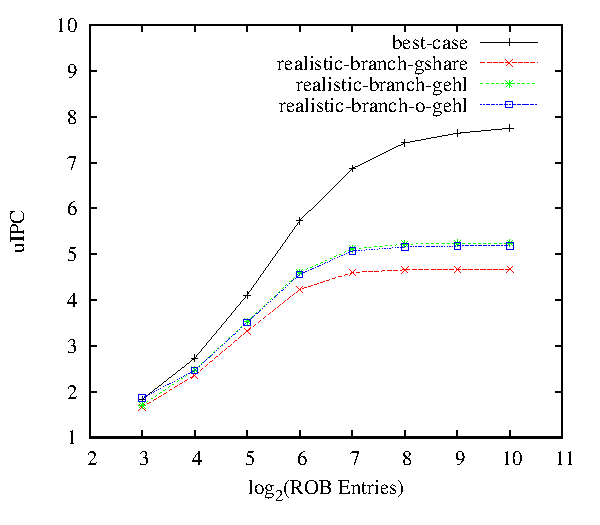
\includegraphics{figs/graph8.pdf}}}
  \subfigure[Standard Deviation of uIPC]{\scalebox{0.8}{\includegraphics{figs/graph8-stddev.pdf}}}

  \caption{Impact of branch predictors on IPC.  On a simulation of a super scalar out of order processor with realistic branch prediction and memory, both GEHL and O-GEHL improve IPC compared to a reference gshare predictor, regardless of the number of entries in the reorder buffer.  `best-case' is a processor with perfect branch prediction and memory scheduling.  All predictors are 64Kbits big and the data was obtained using the long version of the art, gcc, go and sphinx3 traces.}
 \label{fig:ipc}
\end{figure}
